\section{Multimedia}
\textbf{Multimedia}: utilizzo di diversi mezzi che concorrono insieme, solitamente in maniera interattiva, per trasferire informazione. I media hanno caratteristiche e standard differenti per essere catturati, immagazzinati, manipolati e trasmessi.

I segnali devono essere trattati tenendo conto del \textbf{sistema percettivo}. La tecnologia multimediale cerca di simulare il sistema percettivo umano, minimizzando il quantitativo di dati da processare per ottenere un'informazione.

Il trattamento dei media si basa sull'analisi multimodale: essa permette di trarre conclusioni su contenuti di diversi tipi e di individuare stimoli legati a segnali. Per questi scopi devono essere introdotte misure oggettive e soggettive.

Un altro aspetto del multimodale è l'analisi da segnali che provengono da diverse fonti, come i dati fisiologici (ottenuti tramite sensori). 

\section{Segnali}
I segnali possono essere classificati in base a \textbf{dominio} e \textbf{codominio}.

Dominio: 
\begin{itemize}
	\item $D = R$, segnale a tempo (spazio) continuo $x(t),\: t \in R$ (possono assumere tutti i possibili valori reali);
	\item $D = K$, segnale a tempo discreto, $x(t),\: t \in K$ con $K$ numerabile, $K \in \{\dots, t_{-1}, t_0, t_1, \dots\}$. Il numero di valori $t$ può essere comunque infinito.
\end{itemize}

Codominio:
\begin{itemize}
	\item $C = R$, segnale continuo nelle ampiezze;
	\item $C = K$, segnale discreto nelle ampiezze con $K$ numerabile e tipicamente finito $\{x_1, x_2, \dots, x_n\}$.
\end{itemize}

La variabile dipendente è definita sul dominio, quella indipendente sul codominio. I segnali possono essere reali o complessi (parte reale e immaginaria oppure modulo e fase, strettamente in relazione tra loro).

Le ampiezze tipicamente sono un insieme finito di valori, quindi al crescere di $t$ (variabile indipendente, infiniti valori) il \textbf{range} di $s(t)$ (variabile dipendente) sarà limitato, anche se composto da infiniti valori. Il \textbf{passo} (distanza tra un campione e il successivo) dev'essere costante.

La quantizzazione è uno step intermedio della trasformazione tra segnale analogico e digitale, cioè la divisione del tempo (spazio) in passi e l'approssimazione nel dominio. La definizione del passo deve preservare la qualità del segnale, e va stabilita una finestra temporale da considerare.

Le fasi della rappresentazione da analogica a digitale sono \textbf{campionamento}, \textbf{quantizzazione} e \textbf{codifica}.

Bisogna tenere conto di alcuni aspetti delicati, come i limiti di memoria, banda e tempi di processing: questi sono fattori importanti per determinare passo e finestra temporale. I valori cambiano anche a seconda del campo di analisi, per ottenere un'adeguata quantità di informazioni.

\section{Multimedia processing}
Per un efficace trattamento dei segnali multimediali è necessario minimizzare il quantitativo di dati processati, individuando solo quelli strettamente indispensabili. Oltre alla conversione e la compressione ci sono fasi come la memorizzazione e la trasmissione.

L'output è generalmente diverso dall'input: il segnale analogico $x_a$ passa attraverso un campionatore, da cui esce come $x_n$ (non più analogico). L'output $x_q(n)$ contiene un insieme discreto di valori (sottoinsieme del dominio) che poi verrà trasformato in segnale quantizzato $x_q(n)$ e poi in bit.

\begin{figure}[h]
	\centering
	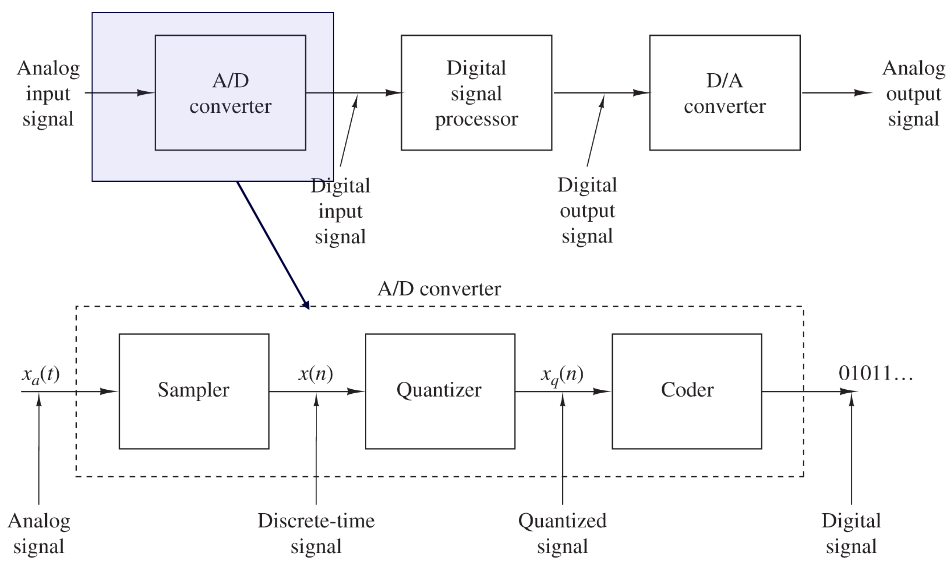
\includegraphics[scale=0.45]{Lezioni/Immagini/conversioneAD}
\end{figure}

Il valore di $x(n)$ è il valore della funzione analogica preso $nT$ volte, dove $T$ è il passo di campionamento. La frequenza è impossibile da ottenere senza la dimensione del passo, ed è legata a quanto velocemente varia il segnale. 

L'obiettivo è capire se esiste una soglia in grado di stabilire se le informazioni vengono perse in base alla dimensione del passo. Avere un'alta \textbf{frequenza di campionamento} significa avere una buona qualità ma un volume elevato dei dati, mentre una bassa frequenza produce fenomeni di aliasing (approssimazione a costante).

Un segnale qualsiasi è rappresentabile come integrali di infiniti termini (seni e coseni) con peso e ampiezza diversi. Tra essi bisogna preservare quello con frequenza massima, per evitare sovrapposizioni e cambiamenti. La scomposizione del segnale è effettuata tramite \textbf{analisi di Fourier}. 

Il \textbf{campionamento} con frequenza massima consente inoltre di riconvertire il segnale digitale in analogico senza perdita di informazione, perché permette la conservazione delle frequenze. \\
La \textbf{quantizzazione}, invece, è un'operazione che comporta sempre perdite, quindi non è reversibile. 

Se il numero di frequenze tende a infinito, com'è possibile individuare la massima? In questo caso si introduce il \textbf{filtering}: l'eliminazione dei valori esclusi da una certa soglia (superiore o inferiore). Un altro motivo del \textbf{filtro anti-aliasing} è l'eliminazione delle frequenze troppo basse.

Un esempio di elaborazione numerica è il filtraggio, l'eliminazione delle frequenze fuori dal range accettabile (filtro passa-basso o alto). I sistemi sono combinazioni di più operatori lineari, quindi nonostante complessi sono scomponibili a causa delle loro proprietà.
